%
% CS6220 Data Mining Project
%
\documentclass[12pt]{article}

%
% Packages
%
\usepackage{amsmath}
\usepackage{caption}
\usepackage{enumerate}
\usepackage[utf8]{inputenc}

\usepackage{clrscode3e}
\usepackage{tikz}

\RequirePackage{graphics}

\usepackage{graphicx}
\graphicspath{ {imgs/} }

%
% Document Settings
%
\setlength{\parskip}{1pc}
\setlength{\parindent}{0pt}
\setlength{\topmargin}{-3pc}
\setlength{\textheight}{9.5in}
\setlength{\oddsidemargin}{0pc}
\setlength{\evensidemargin}{0pc}
\setlength{\textwidth}{6.5in}

\title{Restaurant Recommendations using Yelp}
\author{Manoj Shinde, Tyler Brown, Shohit Bajaj}
\date{ }

% START DOCUMENT
\begin{document}

\maketitle

%\tableofcontents

\begin{abstract}
  When traveling or desiring to experience new food, a person will often seek out restaurant recommendations. 
  The availability of data on restaurant preferences, via Yelp, creates an opportunity for someone to have a more personalized experience. 
  In this project, We have developed a model to predict the star ratings of Yelp Reviews for restaurants using various machine learning algorithms 
  such as Linear Regression, Random Forest Regression. User’s restaurant preferences can be understood via the reviews they write and ratings that 
  they give to a restaurant that they have visited. Supervised learning techniques allow us to predict the rating of unseen restaurants by each user. 
  Restaurant rating predictions allow us to rank which dining experiences are most likely to be well received for each user. 
  \end{abstract}

\section{Introduction}

There are many different types of restaurant experiences due to variation in
personal preferences. A service catering to these personal preferences will
generate value by improving customer convience
\cite{mackay_vandevijvere_xie_lee_swinburn_2017}. Yelp is a popular mobile/web
application that has tons of data on different businesses \cite{Restaura71:online}.
Consumer reviews have been shown to affect restaurant demand. A one-star increase in
Yelp ratings has been linked to a 5-9 percent increase in restaurant revenue
\cite{luca2016reviews}. Consumers do not use all available information and are more
responsive to quality changes that are more visible \cite{luca2016reviews}. It is
not practical for a consumer to go though every rating and review. Sorting through
each recommendation to see which is most relevant is also not practical for the
consumer. We use a supervised learning model to provide value by improving customer
convienence with restaurant recommendations powered by Yelp.

Restaurants on Yelp are given ratings using a five-star scale. We compare two
techniques to solve this multiclass problem. A multinomial logistic regression
is used as a baseline model. We then try to improve our accuracy with the use of
ensemble methods. Data from Yelp has been previously collected and made publicly
available on Kaggle \cite{YelpData59:online}. We demonstrate how to improve
consumer convienence by creating personalized restaurant recommendations with
Yelp data.

Recommendation systems have historically been used in various other disciplines and
are considered quite effective in influencing the decision of a user. In this project
we are trying to make a recommendation based on the rating that a given user would give
to a specific restaurant. Yelp data \cite{YelpData60:online, YelpData59:online} has been
used in a variety of challenges and useful approaches have been well documented in a number of
academic articles \cite{yu2015restaurants, huang2014improving, fan2014predicting,asghar2016yelp}.
Given that the academic community has submitted a number of approaches to predicting
Yelp review ratings \cite{asghar2016yelp, potamias2012warm, fan2014predicting, yu2015restaurants},
we chose to replicate a paper and then extend their analysis. Yu et. al. \cite{yu2015restaurants}
investigate the dataset provided in Yelp Dataset Challenge Round 5 to predict a reviewers
next rating, given their rating history and other contextual factors. We replicate
Yu et. al. \cite{yu2015restaurants} and then extend their paper by developing a model which
generates output that is more consistent with what would be expected by a Yelp user.


\section{Background}
With the advent of websites such as Yelp, customer feedback has become a significant component in business practices. 
In order to maintain and increase their reputations, businesses should adjust their services according to criticism. 
With increasing popularity, Yelp allows users to provide text reviews and assign 1-5 stars to local businesses. 
This platform has collected a large amount of data over the years. As the size of the data continues to grow, 
it would be helpful if we could learn to predict ratings based on review‘s text alone, as free-text reviews are difficult 
for computer systems to understand, analyze and aggregate. This idea can be extended to many other applications where assessment 
has traditionally been in the format of text and quickly assigning a numerical rating is difficult to execute. Examples include 
predicting ratings for TV series or Ted Talks based on news articles or blogs assigning ratings to Netflix videos based on viewers‘ comments.

\section{Methodology}

Our approach was to replicate results which Yu et. al. \cite{yu2015restaurants} found
fruitful and then extend their analysis with an emphasis on real world usability. To meet
these goals, we first conducted a data audit, completed a replication of fruitful results
from Yu et. al \cite{yu2015restaurants}, and then completed an extension of their results.

For this project we have chosen Yelp’s dataset on Kaggle \cite{YelpData59:online}
which is 3GB in size. The dataset has 5,200,000 user reviews, Information on 174,000 businesses,
spanning 11 metropolitan areas in four countries. The dataset has 7 csv files containing data on
different attributes of a business. Our focus is on yelp\_business.csv and yelp\_review.csv where
fields like user\_id, stars, review, category help us in establishing our model.

\begin{figure}[h]
  \caption{Review table Features}
  \centering
  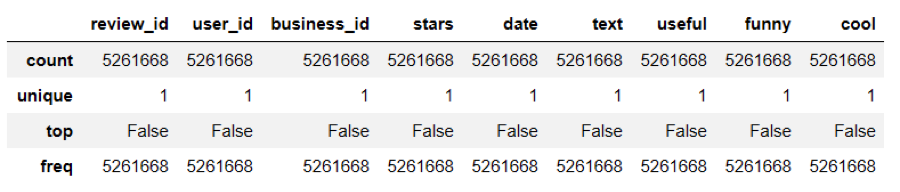
\includegraphics[width=0.75\textwidth]{review_table}
  \end{figure}
  
  \begin{figure}[h]
  \caption{Percent of Zero or NA values per attribute}
  \centering
  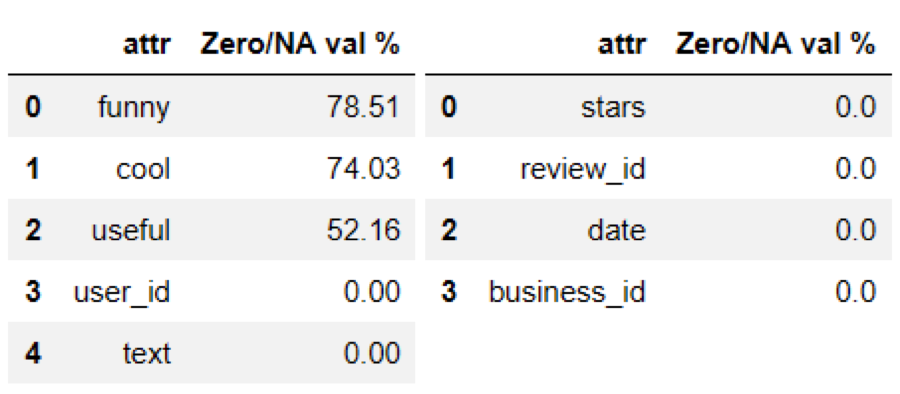
\includegraphics[width=0.5\textwidth]{dataAudit}
  \end{figure}
  
  \begin{figure}[h]
  \caption{Number of Reviews for 1-5 star rating in Dataset}
  \centering
  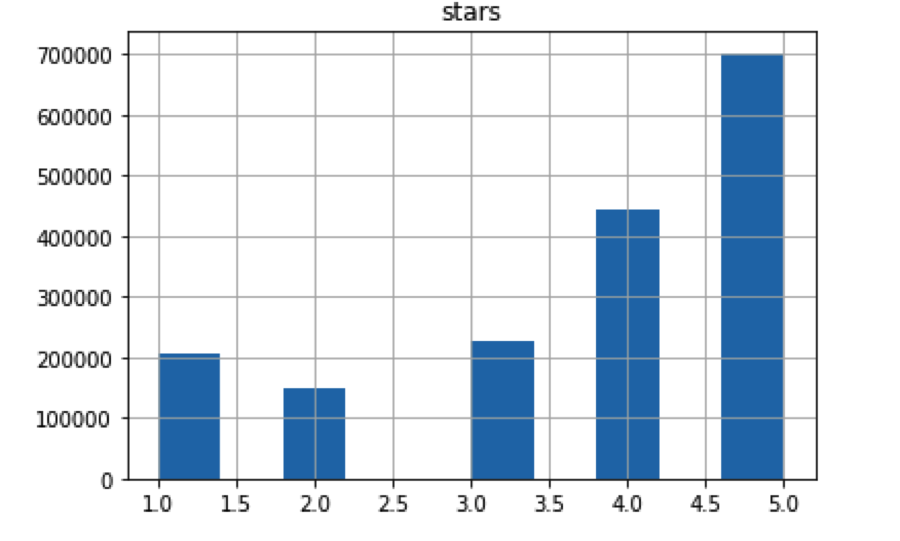
\includegraphics[width=0.5\textwidth]{rating}
  \end{figure}

We evaluated the models in two ways. Models used by Yu et. al. \cite{yu2015restaurants}
were evaluated using Mean Squared Error (MSE). They tried to make their prediction $\hat{R}_{u,i}$
for user $u$ and item $i$ to be as close to $R_{u,i}$, the rating $i$ given by the user $u$.
\[
MSE = \frac{1}{|T|}\sum(R_{u,i} - \hat{R}_{u,i})^2
\]

Our extension of Yu et. al. \cite{yu2015restaurants} used a classification model. In this
case, accuracy was computed by finding the fraction of correct predictions.
\[
accuracy(y, \hat{y}) = \frac{1}{n_{samples}} \sum_{i=0}^{n_{samples} - 1} 1(\hat{y}_i = y_i)
\]
The two-pronged approach was necessary because we extended the analysis by Yu et. al.
\cite{yu2015restaurants} by predicting a discrete rather than continuous variable.

\subsection{Data Audit}

Upon downloading our copy of Yelp Data hosted on Kaggle \cite{YelpData59:online}, we performed
an audit of the data to assess usability and any data quality issues. We found that our
dependent variable, Yelp review stars, contained imbalanced classes. There were considerably
more 4 and 5 star ratings than 1-3 star ratings. The Yelp dataset came to us in several tables.
We created an interactive data visualization to show the relationships between tables by creating
an undirected graph where each node was a table name and each edge showed a foreign key
relationship between nodes. Understanding the data schema was crucial to replicating
Yu et. al. \cite{yu2015restaurants} as well as thinking about and implementing new features.

The second phase of our data audit created tables showing the percentage of NA, blank, and
both NA and blank values in each attribute for each table. This excercise quickly showed us
which tables contained the most usable information for our purposes. For example, the Yelp
Business Attributes table contained several attributes which seemed like they would be
relevant features such as presence of Wifi. Upon conducting an assessment, we found that
the Yelp Business Attributes was almost exclusively populated by NA values. By contrast, the
Yelp Reviews table contained several good attributes but also some unusable attributes
related to the classification of a review as ``funny'', ``cool'', or ``useful''. We found
that conducting an initial data audit up front allowed us to more productively focus our
efforts.

\subsection{Replication of Yu et. al.}

Yu et. al. \cite{yu2015restaurants} predict the number stars for a new review on Yelp.
They compare four distinct models in pursuit of the best prediction: a baseline model,
Linear Regression, Random Forest Regression, and a Latent Factor Model. They applied a
transformation to the dependent variable to normalize each review star for the implicit
noise found in Yelp review data.

\[
\textit{review star} = \textit{review star} - (uAvg + bAvg)/2.0
\]

Utilizing this transformation of the dependent variable, \textit{review star}, they were
able to achieve model results found below in Table 1.

\begin{table}[h]
  \caption{\label{tab:rep-models}Comparison between MSEs for test data (Yu et. al.)}
  \begin{tabular}{|l|l|}
    \hline
    \textbf{Model} & \textbf{MSEs for test data} \\
    \hline
    Baseline & 1.41 \\
    \hline
    Linear Regression & 0.79 \\
    \hline
    Random Forest Regression & 0.64 \\
    \hline
    Latent Factor Model & 1.27 \\
    \hline
  \end{tabular}
\end{table}

Each of the four models used a combination of features described below in Table 2.

\begin{table}[h]
  \caption{\label{tab:features}Model Features}
\begin{tabular}{| l | l |}
  \hline
  \textbf{Feature} & \textbf{Explanation} \\
  \hline
  uRate & average rating stars for each user based on the review stars of the
          training dataset \\
  \hline
  bRate & average rating stars for each business based on the review stars of the training 
          dataset \\
  \hline
  rCount & count of reviews this user had made \\
  \hline
  tlen & lengh of the review text \\
  \hline
  tpol & polarity of the sentiment of the review text \\
  \hline
  tsub & subjectivity of the sentiment of the review text \\
  \hline
  uAvg & average rating stars for each user which can be get from dataset directly \\
  \hline
  bAvg & average rating stars for each business which can be get from dataset directly \\
  \hline
\end{tabular}
\end{table}

We replicated Yu et. al. \cite{yu2015restaurants} with an emphasis on practical application. The
user would expect a review star prediction with discrete values of 1-5. Yu et. al.
\cite{yu2015restaurants} approach the dependent variable as continuous and seek to minimize
the MSE across all new reviews. Their assumptions increase the predictivity of their models but
depart from the output expected by the user. We sought to assess how well the techniques employed
by Yu et. al. would work if model output was more consistent with that expected by a Yelp user.

We excluded the dependent variable transformation utilized by Yu et. al. \cite{yu2015restaurants}
because of the added computational cost of the transformation. We used a dataset of Yelp reviews
which contained about $5 \times$ more records than the dataset used by Yu et. al. \cite{yu2015restaurants} (5,261,668 reviews vs. 990,627 reviews). Substantively, an argument could be made for
adhering to discrete Yelp review star values because these values are expected by Yelp users
when trying to understand where to find a good restaurant. When Yu et. al. \cite{yu2015restaurants}
chose to use regression models and dependent variable transformations then they violated
the expectations of model output by Yelp users because they output review stars as a continuous
rather than discrete variable.

Our approach was to use the top three most performant models by Yu et. al. \cite{yu2015restaurants}
and then add a fourth model of our own which adhered more closely to the review star values
expected by a Yelp user. We replicated the Baseline model, Linear Regression model, and
Random Forest Model.

\subsubsection{Baseline}

Their baseline model used a user's previous average given star (uAvg) to predict their future
reviews' star. For example, when using the training data, an average star for each user
is computed by averaging all of their previous review stars (uAvg). Yu et. al.
\cite{yu2015restaurants} then use those averages to predict the number of review stars in the
test dataset. Only users who exist in the training and test sets were included. This user subset
achieves our goal of predicting how a reviewer will rate their subsequent reviews.

\subsubsection{Linear Regression}

Using features defined in Table 2, we applied the linear regression to the training dataset. The
features are rCount, tlen, tpol, tsub. The label is the review star rating $i$ given by
user $u$. With the features and labels, the linear regression is applied by using
the Scikit-Learn Ordinary Least Squares Regression \cite{sklearnl76:online}. We excluded
additional transformations to the dependent variable due to computational cost.

\subsubsection{Random Forest Regression}

For each review $i$ by user $u$ in the training data, the features are chosen as uAvg, bAvg,
rCount, tlen, tpol, tsub. The label is set to (review star). With the features and labels,
we applied random forest regression by using Scikit-Learn Random Forest Regressor
\cite{32432skl20:online}. In this model, we compared the validation MSE with different
parameters (n estimators and max depth). The evaluation for the model will be discussed the
results section.

\subsection{Extension of Yu et. al.}

The analysis by Yu et. al. \cite{yu2015restaurants} predicts a continuous dependent variable.
A Yelp user would expect restaurant review ratings to be a discrete value between
one and five. Given a 'restaurants you might like' feature, a discrete value makes it easier
for the user to express their preferences by filtering on predicted restaurant review stars,
and other factors like location, to work with Yelp to more quickly find their desired restaurant.
Instead of saying, 'look at these top ten restaurants', Yelp could use our model to say
'search through our restaurant recommendations with these filters'. We see value in making
recommendations an interactive process rather than a presentation of a static list. In order
for the user to experience an interactive process, they will need to be presented with
model output which is intuitive for them. Given these objectives, we used the same features
from Yu et. al. \cite{yu2015restaurants} but implemented a classification model.

\subsubsection{Decision Tree Classifier}

A Decision Tree Classifier \cite{sklearnt25:online} was used to predict the ratings
of a user's future Yelp review. We used several features from Table 2: uRate, bRate, rCount,
tlen, tpol, tsub, uAvg, and bAvg. We tried two distinct strategies to mitigate the class imbalance
in Yelp review data which is skewed towards 4-5 star ratings. The first strategy is to
'balance' the classes by using the values of $y$ to automatically adjust weights inversely
proportional to class frequencies in the input data. Our second approach was to employ
under-sampling. The evaluation of this model will be discussed in the results section.

\section{Code}

The code we used to complete our analysis was all done in Python. We used Jupyter Notebooks
\cite{ProjectJ85:online} to complete each stage of the analysis. The other tool used during
each stage of the analysis was Pandas \cite{PythonDa47:online}.

\subsection{Data Audit}

The data audit included interactive visualization of the Yelp dataset. These visualizations
were achieved using Networkx \cite{NetworkX32:online} to create an undirected network graph,
and Bokeh \cite{Welcomet73:online}  to provide a custom graphic in the style of D3.js
\cite{D3jsData97:online}. 

\subsection{Sentiment Analysis}

Yu et. al. \cite{yu2015restaurants} used the Python package TextBlob \cite{TextBlob35:online}.
It's a package which helps to process text data by providing an API for natural language
processing. For the sentiment analysis tasks (features 'tpol' and 'tsub'), TextBlob returned
a named tuple with float variables representing polarity and subjectivity.

The polarity score is a float number in range of [-1.0, 1.0] with more positive values
representing more positive sentiment. Text expressing negative sentiment may include words
like: 'hate', 'disappointed', 'terrible', etc. Positive sentiment could be expressed with
words like 'wonderful', 'great', etc.

The subjectivity score is also a float number but in range of [0.0, 1.0]. A value of 0.0
indicates the most objective score and 1.0 indicates the most subjective score. A highly
subjective text may use words like 'I', 'we', 'our', etc., with high frequency. Objective
text would use these types of words with a low frequency.

\subsection{Model Implementations}

We used Scikit-Learn for our model implementations \cite{sklearnl76:online, 32432skl20:online,
  sklearnt25:online}. When plotting was used for evaluation, we used
Matplotlib \cite{Matplotl1:online}. 

\section{Results}

Over all models, it was generally found that the scores for extreme end classes i.e. 1 and 5 
were much higher than the scores for middle classes such as 2,3, and 4. This is because it is 
easier to differentiate a clearly negative text from a clearly positive review (binary classification)
but finding polarity of positivity and negativity is more difficult.

\begin{figure}[h]
  \caption{Mean Square Error}
  \centering
  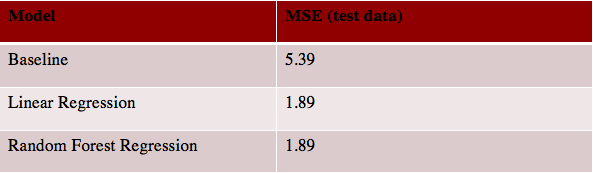
\includegraphics[width=0.5\textwidth]{MSE}
  \end{figure}
  
  We used Decision Tree classifier to predict the outcome between a 1 and a 5 star rating.
  
  \begin{figure}[h]
  \caption{Precision and Recall }
  \centering
  \includegraphics[width=0.5\textwidth]{precisionRecall}
  \end{figure}


\section{Discussion}

We found that a certain model worked better. We found certain patterns
in the data, etc. We also have certain caveats related to the data that
we'll mention here.

\section{Future Work}

Predicted ratings of unseen restaurants can be used to recommend different restaurants to the user based 
on the categories and attributes they prefer. This will enhance their experience on Yelp. 
We can extend our review star prediction to all businesses and not limit it to restaurants. 
We can also try few other models like Ridge Regression, Support Vector Machine, etc. for more accurate results

\section{Conclusion}

We found some things that worked well and other things that worked
less well. There seems to be a positive direction forward taking a
certain approach.


\bibliography{references} 
\bibliographystyle{ieeetr}

\end{document}
